\chapter{Reinforcement Learning}
\section{Introduction}
\side{Reinforcement Learning (RL)}, much like Optimal control, is a mathematical framework that allows us to solve optimal control problems.

In some sense is very similar to Optimal control, but with a very big difference: in Optimal control, you tipically assume to know the analytical/mathematical model of the system that you want to control, whereas in Reinforcement learning you don't.

Either you do not know the mathematical relation between input and state or you may assume that you have a simulator, but you do not have access to code.

Of course, since we have less information it is a much more difficult problem than optimal control, but they share the same structure and some of the key concepts (e.g value function).

A few differene between Reinforcement learning and Optimal control are:
\begin{itemize}
\item Optimal control was born in the control community, whereas reinforcement learning was born in the Computer Science community.
\item RL tries to find the \side{gloablly optimal policy}
\item RL assumes that the dynamics are unknown
\item Initally the community of RL was focused on problems in which the state and the control spaces were finite
\item RL uses different terminology than optimal control, with different names and symbols, even though they represent the same concept
\item tipically RL assumes the dynamics of the system to be stochastic (randomness on the state of the system)

However we will not take this assumption in this module (not a big deal), for sake of simplicity.
\item tipically RL literature focuses on optimizing over an infinite horizon
\end{itemize}

\section{Terminology comparison}

\begin{table}[!h]
\centering
\begin{tabularx}{\textwidth}{|X|X|}
\toprule
\textbf{Reinforcement Learning}&\textbf{Optimal control}\\
\toprule
State $s$& State $x$\\
Action $a$& Control $u$\\
Environment & Plant \\
Reward& Cost function\\
Return & Cost-to-go\\
Maximize&Minimize\\
Value function & Cost to go of a policy\\
Optimal Value function& Value function (Cost to go of the optimal policy)\\
\bottomrule
\end{tabularx}
\end{table}

\section{Framework: Markov Decision Processes (MDP)}
\side{Markov Decision Processes (MDP)} are used to describe the environment in Reinforcement Learning problems, which is assumed to be a \side{fully observable environment} and it has \side{Markov property}.

Markov property means that if you know the current state of the system than knowing the past states does not add any information.
The state tells you everything you know about the system.

Or in other terms: the future is independent on the past given the present.
\[\mathbb{P}(x_{t+1}|x_t) = \mathbb{P}(x_{t+1}|x_1,...,x_t)\]
It can be immediately seen that the system is considered stochastic.

The motion of the state is defined by the \side{State transition probability} which the probability of going from one state $x$ to another state $x'$
\[\mathcal{P}_{xx'} = \mathbb{P}(x_{t+1} = x' | x_t=x)\]
Since in classical Reinforcement Learning you assume that the size of the state space is finite, then you can collect together all the state transition probabilities in a big matrix, called \side{State Transition matrix}.
\[\mathcal{P}=
\begin{bNiceArray}{ccc}
\mathcal{P}_{11}&\Cdots&\mathcal{P}_{1n}\\
\Vdots &\Ddots&\Vdots\\
\mathcal{P}_{n1}&\Cdots&\mathcal{P}_{nn}
\end{bNiceArray}\]
The sum of each row of the matrix will be 1. In deterministic systems $\mathcal{P}$ contains only 0 and 1.

\subsection{Markov Process or Markov Chain}

A \side{Markov Process} is defined by a tuple $<\mathcal{X}, \mathcal{P}>$, where:
\begin{itemize}
\item $\mathcal{X}$ is a finite set of states
\item $\mathcal{P}$ is the \side{state transition probability matrix}
\end{itemize}
A Markov Process is also known as a \side{Markov Chain}

\begin{figure}[!h]
\centering
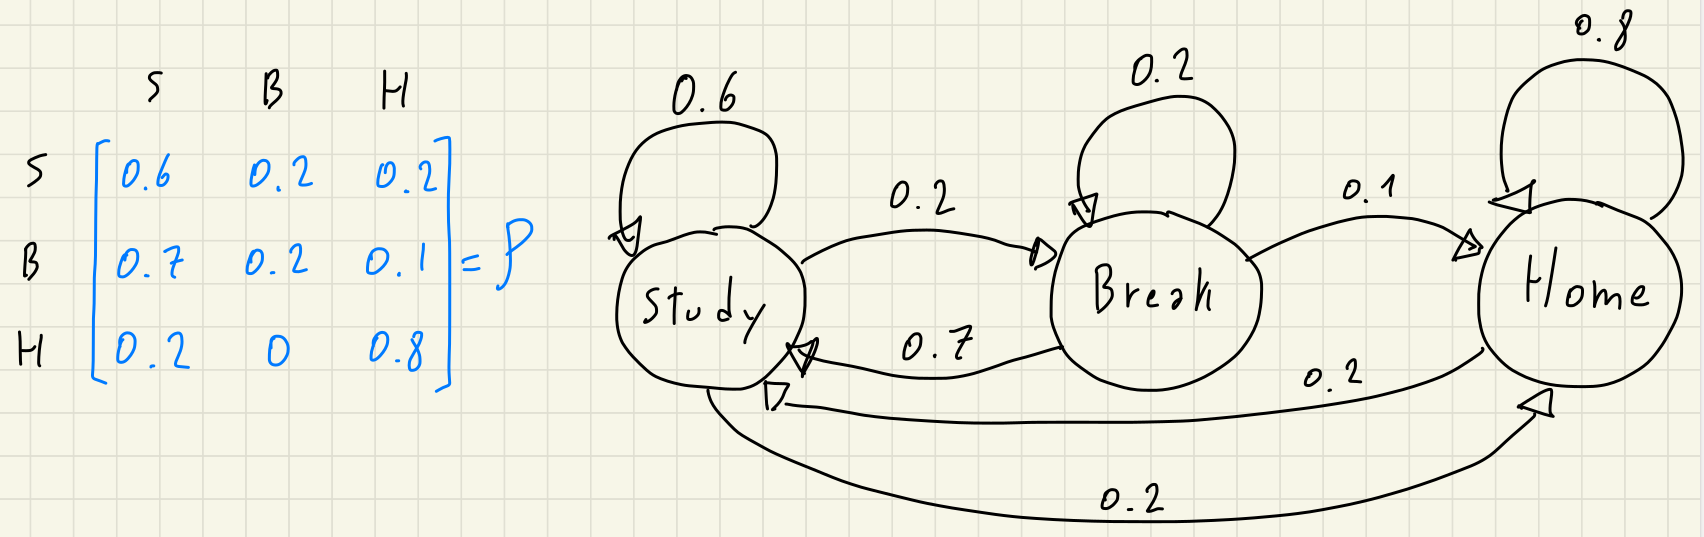
\includegraphics[width=.9\textwidth]{image0301}
\end{figure}

In particular, since $\mathcal{P}$ has all nonegative entries, and it is also \side{irreducible} (associated to a \side{strongly connected graph}), by using \side{Perron-Frobenius theorem} we know that:
\begin{itemize}
\item The largest (in nom) eigenvalue $r$ of $\mathcal{P}$ satisfies the following inequalities:
\[\min_i \sum_j \mathcal{P}_{ij}\le r\le\max_i \sum_{j}\mathcal{P}_{ij}\quad\Rightarrow\quad r = 1\]
which means that the highest eigenvalue of the matrix is $1$
\item All eigenvalues of $\mathcal{P}$ are smaller than $1$.
\[\lambda_i(\mathcal{P})\le 1 \qquad \forall i\]
\end{itemize}

We now have all the tools to try to connect what we have just seen for Markov processes to what we have seen so far for dynamical systems:
\begin{itemize}
\item In Optimal control, since we mostly dealt with \side{deterministic systems}, the dynamic was encoded as:
\[x^+ = f(x)\]
In which, we represented the next state as a function of the state (and  additionally the control inputs).

\item In Markov processes, we can represent the state evolution (aka dynamics) using \side{probability density functions}:
\[\mathbb{P}(x^+|x)\]
\end{itemize}
We therefore can conclude that: 

If a system is deterministic, both approaches can be used (however we will try to use the first approach whenever possible).

\subsubsection{Markov reward process}
A \side{Markov Reward Process} is completely defined by a tuple $<\mathcal{X}, \mathcal{P}, C, \gamma$, where:
\begin{itemize}
\item $\mathcal{X}$ is the state space
\item $\mathcal{P}$ is the probability transition matrix
\item $C$ is the reward (aka cost function)
\[C_x = \mathbb{E}[l_{t+1}|x_t = x]\]
We consider the expected value because we assume that the system is stochastic.
\item $\gamma$ is the \side{discount factor}
\[\gamma \in [0,1]\]
which discounts the cost into the future
\end{itemize}
If we consider the example of Markov Process described before

\begin{figure}[!h]
\centering
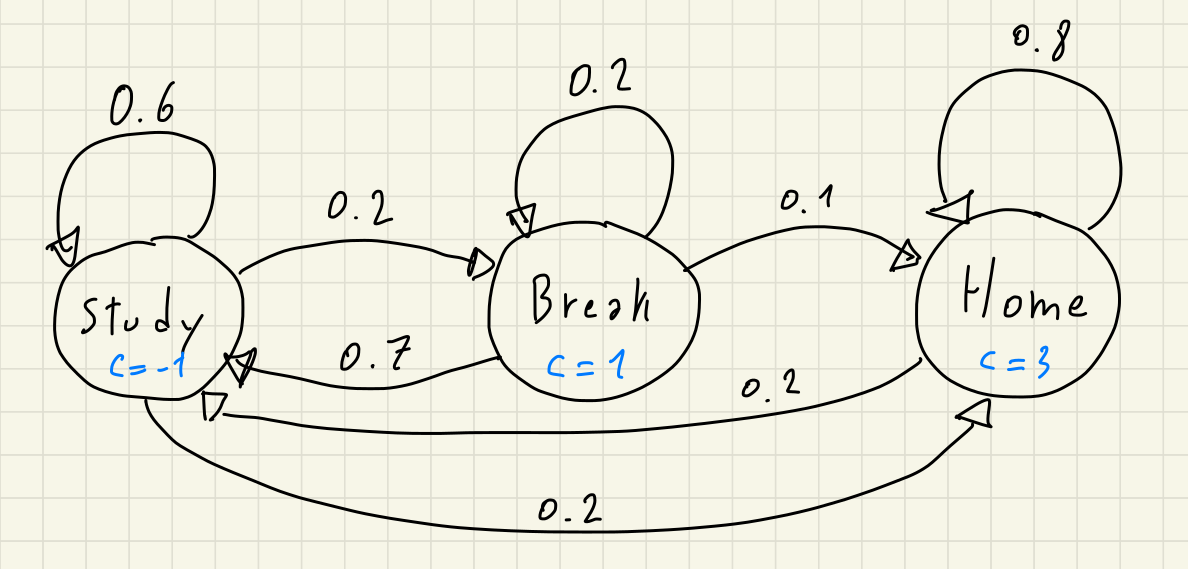
\includegraphics[width = .7\textwidth]{image0302}
\end{figure}
We can translate it into a Markov Reward Process, by simply adding a cost associated with each state. In this situation the lower the cost, the better, since the agent is rewarded for studying and punish for doing breaks and going home.

Regarding the discount factor, the parameter enters into the computation of the cost-to-go (or return), which is nothing more than the total discounted cost from time $t$ to $\infty$:
\[J_t = l_t + \gamma l_{t+1} + \gamma^2 l_{t+2} + ... = \sum_{k=0}^{\infty} \gamma^{k}l_{k+t}\]
Following the above definition, we can infer that $\gamma$ represents the preference for \side{later costs} over \side{immediate costs} (how much you value the future over the present):
\begin{itemize}
\item a value of $\gamma$ close to 0, we obtain a \side{myopic evaluation} (the future has small impact on the decision)
\item a value of $\gamma$ close to 1, we obtain a \side{far-sight evaluation} ($\sim$ optimal control)
\end{itemize}

\begin{center}
\textbf{But why do we need to consider the discount factor?}
\end{center}
\begin{itemize}
\item In order to avoid an infinite cost, since an infinite cost cannot be minimized.
\item There is only a certain degree of uncertainty about the future prediction (reason to favour immediate reward instead of delayed reward).
\item If the cost is associated with some \side{monetary budget}, interest rate and inflation can be modeled using the discount factor. 
\end{itemize}

\subsection{Bellman equation in the context of RL}
Let us define the cost starting from state $x$, as:
\[V(x) = J_t(x_t=x)\]
The \side{Bellman Equation} can be obtained by decomposition of the cost in two parts (assumption: no control input):
\[V(x)=l(x) + \gamma V(f(x))\]
Which can also be represented in matrix form, since RL considers a finite amount of states and control inputs and therefore the Value function and other quantities can be stored in a vector/matrix:
\begin{align*}
\begin{bNiceMatrix}
V(1)\\
\Vdots\\
V(n)
\end{bNiceMatrix}&=
\begin{bNiceMatrix}
l(1)\\
\Vdots\\
l(n)
\end{bNiceMatrix}
+\gamma
\begin{bNiceMatrix}
\mathcal{P}_{11}&\Cdots& \mathcal{P}_{1n}\\
\Vdots&\Ddots&\Vdots\\
\mathcal{P}_{n1}& \Cdots&\mathcal{P}_{nn}
\end{bNiceMatrix}
\begin{bNiceMatrix}
V(1)\\
\Vdots\\
V(n)
\end{bNiceMatrix}\\
&\\
V&=C + \gamma\mathcal{P}V
\end{align*}
The reason why the matrix form and the analytical form of Bellman's equation are equal is because the system is assumed to be deterministic: this means that each row of the transition probability matrix $\mathcal{P}$ will be zero except for the element (which is 1) associated with the next state.

In this way the matrix product between the transition probability matrix with the Value function vector will yield the Value function at the next state, i.e. 
\[V(f(x)) = \mathcal{P}V\]
However, if the system is considered stochastic the matrix formulation still holds whereas the analitical formulation does not make sense since $f(x)$ becomes a probability distribution and therefore cannot be utilized to evaluate the value function.

Moreover, the matrix form is simply a linear system of equation in $V$ and therefore we can ensure that we can explicitly compute it:
\[V=(I-\gamma \mathcal{P})^{-1}C\]
However the Direct solution is only possible for small MRPs. Otherwise, in the case of a large Markov Reward Process with many possible states, then iterative methods can be utilized.

\subsection{Markov Decision Process MDP}
A \side{Markov Decision Process MDP} is uniquely defined by a tuple $<\mathcal{X}, \mathcal{U}, \mathcal{P},C, \gamma>$
where:
\begin{itemize}
\item $\mathcal{X}$ is the state space
\item $\mathcal{U}$ is the control space: (finite) set of control inputs
\item $\mathcal{P}$ is the transition probability matrix
\[\mathcal{P}_{xx'}^u = \mathbb{P}(x_{t+1}=x'|x_T=x, u_t = u)\]
\item $C$ is the cost
\[C_x^u = l_t(x_t=x, u_t=u)\]
\item $\gamma$ is the discount factor
\end{itemize}
 Now that we have introduced the control inputs in the formulation of the system, we can define the notion of \side{policy}: distribution of the control inputs over the states (i.e. a stochastic function).
 
 Given a certain state, you obtain a distribution over all possible control inputs to apply.
 \[\pi(u|x) = \mathbb{P}(u_t=u|x_t=x)\]
 From now on we will assume \side{deterministic policies},i.e.:
 \[u = \pi(x)\]

\subsection{Action-Value Function (Q function)}
The \side{Action-Value Function} is something very similar to the Value function. The Value function is a function of the state and yields the return (cost-to-go) that you will encounter starting from that state and follow a certain policy $\pi$.

Whereas the Action-Value function is an extension of the Value function that takes as input the state and the control input, and yields the cost that you will encounter starting from a state $x$ applying the control $u$ and, from that point onward, following the policy $\pi$.
\[Q^{\pi}(x,u) = J_t(x_t=x, u_t=u, u_{k>t}\sim \pi)\]
We can further decompose the Q-function into two separate terms:
\begin{align*}
Q^{\pi}(x,u) &= l(x,u) + \gamma Q^{\pi}(f(x,u), \pi(f(x,u)))\\
&= l(x,u) + \gamma V^{\pi}(f(x,u))
\end{align*}
where
\[V^{\pi}(x) = Q^{pi}(x,\pi(x))\]

\subsection{Optimal Value Function and Optimal Action-Value Function}
The \side{Optimal Value Function} is the minimum Value function over all possible policies
\[V^*(x) = \min_{\pi}V^{\pi}(x)\]
SImilarly we can define the \side{Optimal Action-Value Function}:
\[Q^*(x,u) = \min_{\pi}Q^{\pi}(x,u)\]
And as a result the \side{Optimal policy} is defined as:
\[\pi^* \le \pi \qquad \forall \pi\]
where
\[\pi\le\pi'\qquad\text{if } V^{\pi}(x) \le V^{\pi'}(x)\quad \forall x \in \mathcal{X}\]

One possible way of computing the optimal policy, which is often used in reinforcement learning, is to first:
\begin{itemize}
\item Minimize the Action-Value Function $Q^*$ over u:
\begin{align*}
\pi^*(x) &= \argmin_{z\in\mathcal{U}}Q^*(x,z)\\
&= \argmin_{z\in\mathcal{U}} l(x,u) + \gamma V^*(f(x,u))
\end{align*}
But by assumption we do not know the dynamics $f(x,u)$, that is why we utilize the Q function.
\end{itemize}

Therefore, if we know $Q^*(x,u)$, then we immediatly have the optimal policy.

\subsection{Bellman Optimality equation}
The \side{Bellman Optimality equation} is the optimal version of the Bellman equation:
\begin{align*}
V^*(x) &= \min_u Q^*(x,u)\\
&= \min_u l(x,u) + \gamma V^*(f(x,u))
\end{align*}

which implies that:
\begin{align*}
Q^*(x,u)&=l(x,u) + \gamma V^*(f(x,u))\\
&= l(x,u) + \gamma \min_{u'} Q^*(f(x,u),u')
\end{align*}
We obtained:
\begin{itemize}
\item A nonlinear systems (because a minimization is non linear)
\item No closed-form solution
\item Iterative algorithm are utilized to find the solution
\end{itemize}

\section{Model Based Control}
\subsection{Dynamic Programming}
Before diving deep into Reinforcement Learning algorithms we need to understand the algorithmic foundation of RL, which is \side{Dynamic Programming}.

We have already discussed Dynamic Programming in the context of Optimal Control, but as we will see in this section RL rely much more on Dynamic Programming than Optimal control.

However, note that Dynamic Programming is not yet RL since, in DP, you assume that you have full knowledge of the model (in our case of the MDP).

In the context of Dynamic Programming there are two classes of problems that we can deal with:
\begin{enumerate}
\item \side{Prediction}

In a prediction problem you already have a MDP and a policy (function that tells you the control input to apply in each state), and you want to evaluate how good that policy is (i.e. the value function associated with that policy).

Formally:
\begin{itemize}
\item Input: MDP $<\mathcal{X},\mathcal{U}, \mathcal{P},C, \gamma>$ and policy $\pi$
\item Output: Value function $V^{\pi}$ (not the optimal one)
\end{itemize}
\item \side{Control}

In a control problem you already have a MDP and you want to find the \side{optimal control policy} (and tipically the \side{optimal value function} associated to it).

Formally:
\begin{itemize}
\item Input: MDP
\item Output: optimal value function $V^*$ and optimal policy $\pi^*$
\end{itemize}
\end{enumerate}

\subsubsection{Difference between Finite and Infinite Horizon}
What we have discussed when talking about DP is the case of \side{Finite Horizon}, so we assumed an horizon over which we want to optimize was finite. What we are gonna see  instead is the application of DP with \side{Infinite Horizon}.

The main reason of this change in approach is due to the fact that in Optimal control you usually deal with a Finite Horizon problem, whereas in RL most of the literature deals with Infinite Horizon problems; as a consequence, we need to base our algorithms on different versions of DP (we will see that this changes the way the algorithm behaves).

\begin{itemize}
\item Finite horizon
\begin{itemize}
\item Theory is simpler (you start fro the last time step and you already now the Value function associated with it)
\item mostly used in Optimal Control
\item the policy and Value function depends on time, because depending on how much time you have left, the optimal thing to do might be different.

\begin{figure}[!h]
\centering
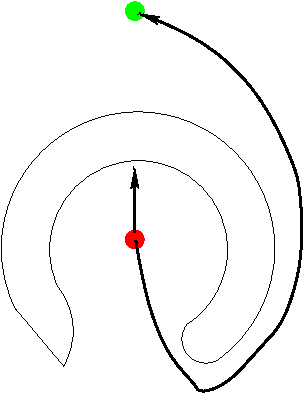
\includegraphics[width = .3\textwidth]{image0303}
\caption{With a finite horizon (if not much time is left to reach the target) the best thing the algorithm can do is get as close as possible to the goal point, with an infinite horizon the algorithm has enough time to find the path that reaches the goal position}
\end{figure}
\end{itemize}
\item Infinite horizon
\begin{itemize}
\item theory is more complex, but it is elegant (even though the theory is complex, this kind of complexity in the end disappears resulting in a beautiful and simple algorithm, sometimes simpler than the version with finite horizon)
\item mostly used in RL
\item the policy and Value function are stationary (independent of time)
\item good approximation of long finite horizon problems
\end{itemize}
\end{itemize}

\subsubsection{Bellman operators}
Before diving deep into the DP algorithms with infinite horizon we need to introduce the notion that we will use in defining them:
\begin{itemize}
\item \side{Bellman (expectation backup) operator} $T^{\pi}$.
\[T^{\pi}(V) = C^{\pi} + \gamma\mathcal{P}^{\pi}V\]
The input is the Value function (or vector of Value functions) and the output is another Value function.
\item \side{Bellman optimality (backup) operator} $T$.
\[T(V) = \min_{u\in\mathcal{U}} C^u + \gamma\mathcal{P}^uV\]
In this case you do not have a policy to follow but you minimize over all possible control inputs (for each possible state):
\[(TV)(x) = \min_{u\in\mathcal{U}} l(x,u) + \gamma V(f(x,u))\qquad\forall x \in \mathcal{X}\]
\end{itemize}

The expression are basically the Bellman optimality principle equation:
\[V_k(x) = \min_{u} l(x,u) + V_{k+1}(f(x,u))\]

\subsection{Prediction}
\subsubsection{Iterative Policy Evaluation}
The \side{Iterative Policy Evaluation} algorithm can be defined as follow:
\begin{itemize}
\item Problem: Given a MDP and a given policy $\pi$. Evaluate the given policy.
\item Solution: Apply iteratively Bellman expectation operator:
\[V_{k+1} = l(x,\pi(x)) + \gamma V_{k}(f(x,\pi(x)))\qquad \forall x \in \mathcal{X}\]
This means that we compute a sequence of approximation of the Value function, where each approximation is computed from the previous approximation.

The recursive application of the Bellman operator can be represented in a shorter notation:
\[V_{k+1} = T^{\pi}V_k\]

In this case $k$ refers to the iteration of the algorithm not the time step since it does not depend on time
\end{itemize}

The algorithm goes as follow:
\begin{enumerate}
\item Start with an arbitrary Value function $V_0$
\item Iterate using
\[V_{k+1} = T^{\pi}V_k\]
\item Guarantee to converge to $V_{\pi}$, since
\[\lim_{k\to\infty} V_k = V_{\pi}\]
In practice you will converge before infinity.
\end{enumerate}

\begin{proof}
Starting from:
\[V_{k+1} = T^{\pi}V_k\]
\begin{enumerate}
\item We first need to prove that $T^\pi$ is \side{contracting},  i.e. the distance (measured using the $L_{\infty}$ norm) between two value functions $V$ and $Z$ decreases if you apply the Bellman operator.
\begin{align*}
\norma{T^{\pi}V - T^{\pi}Z}_{\infty} &= \norma{\cancel{C^{\pi}}+\gamma \mathcal{P}^{\pi}V - \cancel{C^{\pi}} - \gamma \mathcal{P}^{\pi}Z}_{\infty}\\
&= \gamma \norma{\mathcal{P}^{\pi}(V-Z)}_{\infty}\\
&\le \gamma \norma{V-Z}_{\infty}
\end{align*}
Because each row of $\mathcal{P}^{\pi}$ sums to 1.

In the specific case of a deterministic problem, by applying the transition probability matrix only changes the order of the difference of Value functions not the norm.

\item Secondly we would like to prove that given an arbitrary Value functin $V_0$ and the value associated with the policy $V_{\pi}$, $V_{k}\to V_{\pi}$ as $k\to\infty$
\begin{align*}
\norma{V_k - V_{\pi}}_{\infty} &= \norma{T^{\pi}V_{k-1} - T^{\pi}V_{\pi}}_{\infty} \\
&\le\gamma\norma{V_{k-1} - V_{\pi}}_{\infty} \\
&\le \gamma^2 \norma{V_{k-2} - V_{\pi}}_{\infty}\\
&\le ...\\
&\le \gamma^k \norma{V_{0}-V_{\pi}}_{\infty}
\end{align*}
Which states that $V_{k}$ converges to $V_{\pi}$ at \side{geometric rate}, and the geometric rate is defined by the discount factor $\gamma \in [0,1]$

Note that $V_{\pi}$ is invariant, therefore 
\[V_{\pi} = T^{\pi}V_{\pi}\]
\item Prove $V_{\pi}$ is unique fixed point of $T^{\pi}$.

Assume $V$ and $Z$ are both fixed points of $T^{\pi}$, i.e.
\[T^{\pi}V = V\qquad T^{\pi}Z = Z\]
By doing so we are going to prove that the only way that could be two of them is if they are equal $V=Z$
\begin{align*}
\norma{T^{\pi}V - T^{\pi}Z}_{\infty} &\le \gamma \norma{V-Z}_{\infty}&\text{Because }T^{\pi}\text{ is contracting}\\
\norma{T^{\pi}V - T^{\pi}Z}_{\infty} &= \norma{V - Z}_{\infty} &\text{Because }V,Z \text{ are fixed points}\\
\gamma\norma{V-Z}_{\infty} &\ge \norma{V-Z}_{\infty} \quad\Rightarrow\quad \norma{V-Z}_{\infty} &\text{Because } \gamma <1
\end{align*}
Therefore the only way the inequality holds is if and only if $V=Z$, which means that the only way these two points are both fixed is if they are the same point.
\end{enumerate}
\end{proof}

\subsection{Control}
\subsubsection{Policy Iteration}
The \side{Policy Iteration} algorithm can be defined as follow:
\begin{itemize}
\item Problem: Given an MDP, find the optimal policy $\pi^*$
\end{itemize}

The algorithm goes as follow:
\begin{enumerate}
\item Start with an arbitrary policy $\pi_0$
\item Iterate for $k = 0...\infty$ 
\begin{itemize}
\item Evaluate the policy $\pi_k \Rightarrow V^{\pi_k}$ (bottleneck)
\item Improve the policy acting greedily w.r.t. $V^{\pi_k}$:
\[\pi_{k+1}(x) = \argmin_{u} l(x,u) + \gamma V^{\pi_k}(f(x,u))\qquad \forall x \in \mathcal{X}\]
The minimization is computed by evaluating the argument for all possible $u$, you store the results in a vector and then you compute the minimum of the vector (\side{minimization by enumeration}). 
\end{itemize}
\end{enumerate}

This algorithm always converges to the optimal policy $\pi^*$
\[\lim_{k\to \infty} \pi_k = \pi^*\]
We can show that this convergence works:
\begin{proof}
The way you show that policy iteration converges to the optimal policy is by showing that at each iteration of the algorithm, you obtain a policy that is better than the previous one, i.e,:
\[\pi_{k+1}\le\pi_k\quad \forall k \qquad \iff \qquad \pi' \le \pi\]
Here the inequality applied to the policies means that the value function associated to a policy is always less than or equal to the value function associated to another policy.
\begin{align*}
\pi'(x) =&\argmin_u [l(x,u) + \gamma V^{\pi}(f(x,u))]\\
& \min_u [l(x,u) + \gamma V^{\pi}(f(x,u))]\le l(x,\pi(x)) + \gamma V^{\pi}(f(x,\pi(x)))\\
\end{align*}
Where :
\begin{itemize}
\item the lhs of the inequality is the cost we get by following $\pi'$ for first step and then following $\pi$ (because we are using $V^{\pi}$ to estimate the tail of the cost)
\item the rhs of the inequality is the cost following $\pi$ 
\end{itemize}
Then  I need to find a way to iterate in order to show that following $\pi'$ is better than to follow $\pi$, and the way we are going to do it is by using the Q function:
\[Q^{\pi}(x,\pi') = \min_{u} [Q^{\pi}(x,u)]\le Q^{\pi}(x,\pi(x)) = V^{\pi}(x)\]
\begin{align*}
V^{\pi}(x) &\ge \min_u [l(x,u)+\gamma V^{\pi}(f(x,u))]&V^{\pi}(x) \ge Q^{\pi}(x,\pi')\\
&\ge l(x,\pi') + \gamma Q^{\pi}(x', \pi')&x'\triangleq f(x,\pi')\\
&= l(x,\pi') + \gamma l(x',\pi') + \gamma^2 V^{\pi}(x'')&\text{Cost following }\pi'\text{for 2 steps and then }\pi\\
&\ge l(x,\pi') + \gamma l(x', \pi') + \gamma^2 Q^{\pi}(x'', \pi')&\pi' \text{ for 3 steps}\\
&\ge \sum_{i=0}^{\infty} \gamma^i l(x^{(i)}, \pi') = V^{\pi'}(x)&
\end{align*}
\[V^{\pi} \ge V^{\pi'} \iff \pi'\le \pi\]
\end{proof}

\subsubsection{Modified policy iteration}
Since most of the computation time of the policy iteration algorithm is spent evaluating the policy, we can introduce a variation of the algorithm called \side{Modified policy iteration} algorithm, based on the idea that maybe we do not need to evaluate the policy exactly, but instead compute an approximation of its value function.
\begin{itemize}
\item Use $m_k$ policy evaluation iterations to compute $V^{\pi_k}$.

Under some mild assumptions even this algorithm converges to $V^*$.
\item Of course if we take $m_k = \infty$ we recover the policy iteration algorithm.
\item If we take $m_k = 1$ we obtain the \side{Value Iteration} algorithm.

Every time you update $V$ you use a policy that is greedy w.r.t. $V$.
\end{itemize}

\subsubsection{Value iteration}
In the \side{Value iteration} algorithm you do not keep track of the policy but instead you store in memory the Value function.

So you try to compute the optimal value function and then, only at the end, when you have obtained the optimal value function, you compute the policy.
\begin{enumerate}
\item Start with an arbitrary estimation of the Value function $V_0$
\item Iterate for $k = 0,...,\infty$
\begin{itemize}
\item For all the states $x\in\mathcal{X}$ 

You update the Value function:
\[V_{k+1}(x) = \min_u l(x,u) + \gamma V_k(f(x,u))\]

This for loop can be simply rewritten as:
\[V_{k+1} = TV_k\]
\end{itemize}
\item $V_k$ is guaranteed to converge to the optimal value function $V^*$
\[\lim_{k\to\infty} V_k = V^*\]
\item Once you have obtained the optimal value you can compute the optimal policy $\pi^*$
\[\pi^* = \argmin_u l + \gamma V^*\]
\end{enumerate}


\section{Model Free Prediction}
In this section we dive deep into the decision process of Reinforcement Learning: in fact, so far, we assumed that the MDP is given and well defined (as well as the dynamics of the system) and we were able to exploit it in order to find the optimal policy or the value function given a fixed policy.

From now on, we will start relaxing this assumption, i.e. we do not know the MDP and we can only choose the control inputs and observe state and cost.\\
However, in this section we will focus on prediction not control, which will be our foundation for doing control in the next sections.

With prediction, we mean that the policy is assumed to be given (\side{fixed policy}) and we just want to find the value function associated with that policy.\\
This vaguely reseamble the DDP approach \side{policy evaluation}, which turned out to be the basis for doing policy iteration (first algorithm that we look at in order to find the optimal policy).

Formally:
Problem: Find the value function of unkown MDP by acting (choosing the action/control input) and observing. 

In order to solve the problem there are two main approaches, which are the extreme of a more general approach.
\begin{enumerate}
\item \side{Monte Carlo (MC)}

The key idea of this method is really simple: if I would like to estimate the value of a state
\begin{itemize}
\item I start from that state
\item I run my policy
\item Collect all the costs until the end of the episode (all the episodes must end)
\item I sum all the costs and that is going to give me an estimate of the value of that state.
\end{itemize}

Tipically in RL we assume that the MDP and/or the policies and/or the costs are stochastic, so I would have to repeat this process several times. By taking the average over the different summations, we would obtain the mean/estimate.

In summary: the value of a state can be estimate from the mean of the cost-to-go, however it can only be applied to \side{episodic MDPs} (i.e. all episodes must end).
\item \side{Temporal Difference Learning TD0}
\end{enumerate}


\subsection{Monte Carlo Policy Evaluation}
The goal of \side{Monte Carlo Policy Evaluation} is to learn the value of a given policy $V_{\pi}$ from episodes of experience under policy $\pi$.

By \side{episode} we mean one execution of the policy from a \side{starting state} to a \side{terminal state}.

As a consequence, each episode will be a list of state, control and cost for each step:
\[x_1, u_1, l_1 , ... , x_k \sim \pi\]
As mentioned before we can compute the Cost-to-go, i.e. the total discounted cost:
\[J_t = l_t + \gamma l_{t+1} + ... + \gamma^{T-1} l_{t + T-1}\]
and then once we have the cost-to-go for each time we can use it to estimate the value function, by means of \side{expected cost-to-go} under policy $\pi$:
\[V^{\pi}(x) = \mathbb{E}[J_t | x_t = x]\]
Since we are using the expected value operator we are implicitly assuming some stochasticity in MDP or in the policy or in the cost.

In case of deterministic processes, you only need one sample (no need to apply the expected value operator).

Summary:
Monte Carlo policy evaluation estimates $V^{\pi}$ as the average cost-to-go.

The algorithm implementation has two versions, depending on when to start accumulating the cost: if you encounter a state multiple times you are gonna get different values depending wheter you start accumulating the cost the first time you meet that state or every time you meet the state.
\begin{itemize}
\item \side{First-visit MC policy evaluation}

The first time that a state $x$ is visited in an episode:
\begin{enumerate}
\item Increment a counter (how many times have you met that state)
\[N(x) \leftarrow N(x) + 1\]
\item Increment the total cost (in order to compute the cost-to-go)
\[C(x)\leftarrow C(x) + J(x)\]
\item Estimate value as the average cost-to-go
\[V(x) \leftarrow \cfrac{C(x)}{N(x)}\]
\end{enumerate}
These three steps are repeated only the first time you encounter a state (no increment happens if you encouter the same state).

This method works by exploiting the \side{law of large numbers}
\[V(x)\rightarrow V^{\pi}(x)\qquad\text{as }N(x)\rightarrow\infty\]
\item \side{Every visit MC policy evaluation} 

the counter and total cost are incremented every time a state is visited.
\end{itemize}

Since computing the mean each time is annoying what is very often done is \side{Incremental MC updates}: update the mean incrementally.
\begin{align*}
V_N &= \cfrac{1}{N}\sum_{j=1}^N J_i&\text{decompose summation}\\
&=  \cfrac{J_N +\sum_{j=1}^{N-1} J_j}{N}&V_{N-1} = \cfrac{1}{N-1}\sum_{j=1}^{N-1} J_j\\
&= \cfrac{J_N + (N-1)V_{N-1}}{N}\\
&= V_{N-1} + \cfrac{1}{N}(J_N - V_{N-1})  
\end{align*}
In this way we can compute the new mean starting from the previous one.
However as $N$ becomes large the influence of the increment tends toward zero. However, this is an undesirable effects especially in non-stationary environments than new samples will have a lower effect on the estimate of the value.

That is why, very often, instead of dividing for $N$ a fixed value is used (it an be useful to track a running mean, i.e. forget old episodes):
\[V(x) \leftarrow V(x) + \alpha (J - V(x))\]
In this view $\alpha$ is how fast we are going to update based on the most recent sample.

\subsection{Temporal Difference Learning - TD0}
\side{Temporal Difference Learning (TD0)} is an alternative method to MC, and it estimates the cost-to-go by using the \side{1-step look ahead}, i.e.:
\[V(x_t) \leftarrow V(x_t) + \alpha_t (l_t + \gamma V(x_{t+1}) - V(x_t))\]
where:
\begin{itemize}
\item{\makebox[5cm]{$l_t + \gamma V(x_{t+1}) - V(x_t)$\hfill} is the }\side{TD error}
\item{\makebox[5cm]{$l_t + \gamma V(x_{t+1})$\hfill} is the }\side{TD target}, which is out estimated cost-to-go
\end{itemize}

It is now very useful to compare it to MC using the inremental update:
\[V(x_t) \leftarrow V(x_t) + \alpha_t (J_t - V(x_t))\]
where 
\[J_t \approx l_t + \gamma V(x_{t+1})\]
where rhs reminds us of Bellman equation.
The key intution is instead of collecting all the costs starting from the state till the end of the episode, I only see 1 cost and in order to estimate the tail of the cost-to-go I use the estimate of the value function.
Whereas MC target is based on what we observe from the environment.

Policy evaluation is TD(0) with $\alpha_t = 1$ and sampling all states uniformly.

The properties of TD(0) are:
\begin{itemize}
\item TD(0) is a \side{stochastic approximation algorithm}.
\item Since Bellman operator has a unique fixed point, then if TD(0) converges (and all states are sampled infinitely often) then it must converge to $V^{\pi}$.
\item Convergence is guaranteed if step-size sequence satisfies \side{Robbins-Monro (RM) conditions}:
\[\sum_{t = 0}^{\infty} \alpha_t = \infty\qquad \sum_{t = 0}^{\infty}\alpha_t^2 <\infty\]
which means that cannot tend to zero and how much you update should tend towards zero (you need to update by smaller and smaller amounts to ensure convergence), e.g.
\[\alpha_t = \cfrac{\bar{\alpha}}{t}\]
\item In practice, I constant $\alpha$ is sufficient in most of the time: the algorithm might converge anyway even if we do not have any guarantee of convergence.
\end{itemize}

\subsection{Comparison betweeen MC and TD0}
\begin{table}[!h]
\centering
\begin{tabularx}{\textwidth}{|X|X|}
\toprule
\textbf{MC}&\textbf{TD}\\
\midrule
$\bullet$ Must wait until end of episode to know cost & $\bullet$ can learn after every step\\
$\bullet$ only works for episodic environments& $\bullet$ works in non-terminating environments\\
$\bullet$ MC target (cost-to-go) is unbiased estimate of $V_{\pi}(x_t)$, given that it is an observation& $\bullet$ TD target is a biased estimate of $V_{\pi}(x_t)$, given that it is based on the current estimation of the value (which can be arbitrary bad)\\
$\bullet$ Higher variance estimate of $V_{\pi}(x_t)$, given that $J_t$ contains the cost of each transition and at each transition some stochasticity exists.

Therefore more variance is added to the equation at each transition & $\bullet$ Lower variance estimate of $V_{\pi}(x_t)$, given that it has only one transition (the estimate of the tail is not stochastic)\\
\bottomrule
\end{tabularx}
\end{table}

In practice, it depends which one perform better:
\begin{itemize}
\item MC has high variance, zero bias:
\begin{itemize}
\item very good convergence properties (given by the fact that has zero bias)
\item works well even with function approximation.

At a certain point in order to scale up this algorithm to be able to work with real system in continuous time, you cannot accept anymore working with arrays, given that the size will grow too much. What you need to do, as a consequence, to make it work with large systems is to use function approximation e.g. neural networks (the value functino will be a NN: instead of changing values inside the vector, we are going to change the weights of the NN).
\item Not very sensitive to initialization.
\item Simple to understand and use
\end{itemize}
\item TD has low variance, some bias:
\begin{itemize}
\item Usually is more efficient than MC
\item converges to $V_{\pi}(x_t)$ faster
\item but convergence is not guaranteed if you are using functino approximation
\item more sensitive to the initial guess/value
\end{itemize}
\end{itemize}


\subsection{Bootstrapping and Sampling}

We can describe the algorithms that we have seen so far with a table.
\[
\begin{NiceArray}{cWc{4cm}c|Wc{4cm}Wc{4cm}}
\Block{3-3}{\diagbox{\qquad\text{Sampl.}\vspace{2mm}}{\vspace{2mm}\text{Bootstr.}\qquad}} &&&&\\
&&&\text{No} & \text{Yes}\\
&&&&\\
\hline
&&&&\\
&\text{No} && \text{Exhaustive \newline Search} & \text{DP}\\
&&&&\\
&\text{Yes} &&\text{MC}& \text{TD}\\
&&&&
\end{NiceArray}
\]
where:
\begin{itemize}
\item \side{Bootstrapping}: updates of the quantity that you are trying to estimate involve an estimate (TD0).

The TD target is computed based on the current estimate of the value function.
\item \side{Sampling}: updates sample an expectation (MC).

Informally we are collecting samples of a quantity and computing the mean: we are approximating an expectation using the mean over a few samples.
\end{itemize}

\subsection{n-Step return}
Let us know take a step further and see how we can generalize MC and TD0 to a more general class of algorithms which actually include MC and TD0 as special cases.

We can do that by introducing the idea of \side{n-Step return}, which is instead of collecting just one transition (i.e. one cost) and summing  to this cost the discount times the estimate of the value at the next state, we can generalize this concept to several steps:
\begin{align*}
n=1 &\qquad J_t^{(1)} = l_t + \gamma V(x_{t+1})&TD0\\
n=2 & \qquad J_t^{(2)} = l_t + \gamma l_{t+1} + \gamma^2 V(x_{t+2})&\\
\vdotswithin{n=2} &\qquad\vdotswithin{J_t^{(2)}}&\\
n\hphantom{\,\,2} & \qquad J_t^{(n)} = l_t + \gamma l_{t+1} + ... + \gamma^{n-1} l_{t+n-1} + \gamma^{n}V(x_{t+n})&\\
\vdotswithin{n}\hphantom{\,\,2}&\qquad\vdotswithin{J_t^{(n)}}&\\
n=\infty&\qquad J_t^{(\infty)} = l_t + \gamma l_{t+1} + ... + \gamma^{T-1} l_{t+T-1}&MC
\end{align*}

And the update equation will be simply (\side{n-step TD learning}):
\[V(x_t) \leftarrow V(x_t) + \alpha_t (J_t^{(n)} - V(x_t))\]

In this way we introduced a new kind of algorithm to do prediction and estimating the value of a given policy where instead of using the 1-step cost-to-go (TD0) or the infinite-step cost-to-go (MC), we can use a more general n-step estimation of the cost-to-go which is going to give us some algorithms which are an inbetween MC and TD0.

So, of course, an algorithm which is an hybrid between these two extreme approaches, will give us something inbetween the properties of MC and TD0: e.g. in terms of bias-variance trade-off we can imagine that as we utilize a higher value of $n$ we are going to get more and more variance in the estimate and lower and lower bias.

In other terms we can make TD0 tends towards the property of MC by tuning the $n$ parameter to the values that we want.
In fact the best performance are achieved neither with MC nor with TD0 but for a value of $n$ inbetween.

\subsection{TD($\lambda$)}
We can do something a bit more convoluted: since we have a family of algorithms (one for each value of $n$) and we do not know which one to use, what if we use all of them?\\
So we use all the estimates of the cost to go by putting them together with some weights, and that is exactly what \side{TD($\lambda$)} does.

So $TD(\lambda)$ is a new algorithm for doing prediction where you combine all the n-step costs-to-go $J_t^{(n)}$ together by using weights of the form:
\[(1-\lambda)\lambda^{n-1}\]
As a consequence, the \side{TD($\lambda$) target} is given by the expression:
\[J_t^{\lambda} = (1-\lambda) \sum_{n=1}^{\infty} \lambda^{n-1} J_t^{(n)}\]
This means that the algorithm is going to use an higher weight for the first estimate of the cost to go ($n=1$) and a smaller and smaller weight for the remaining n-step costs-to-go estimation.

The reason of the $(1-\lambda)$ premultiplication is just for normalizing the weights, given that the summation of all the weights must be equal to $1$ (otherwise you are not taking an average anymore)
\[\sum_{n=1}^{\infty}\lambda^n = \cfrac{1}{1-\lambda}\qquad \text{with: }0<\lambda<1\]
The TD($\lambda$) algorithm can be seen in two different fashions: \side{forward view} and \side{backward view}.
\begin{itemize}
\item the forward view is much easier and more intuitive to think of and analyze in terms of theoretical properties but is very tricky to implement
\item the backward view is much more convoluted and harder to analyze but this is what makes the implementation of this algorithm easier.
\end{itemize}

\subsubsection{Forward view}
With the forward view, the value is updated as usual:
\[V(x_t)\leftarrow V(x_t) + \alpha_t (J_t^{\lambda} - V(x_t))\]
The problem with the implementation of this algorithm is that we can only learn from \side{complete episodes} (as in MC).

That is the reason why people have derived the backward view of TD($\lambda$).
 
\subsubsection{Backward view}
The Backward view of TD($\lambda$) is a little more criptic and hard to understand how it works, but actually, given some assumption, it will be equivalent to the Forward view of TD($\lambda$).

However, this view of the algorithm allows us to updates the estimate at each transition without waiting till the very end.

In order to implement the Backward view of TD($\lambda$) we need to introduce new quantities called \side{Eligibility traces}, defined by the following two equations:
\begin{align*}
e_0(x) &= 0&\text{Initialize Eligibility trace of each state to 0}\\
e_t(x) &= \gamma\lambda e_{t-1}(x) + 1(x_t=x)&\text{if you meet state }x\text{ the eligibility trace increase by 1}
\end{align*}
Once the state is met, then the eligibility trace will decrease.

These quantities measure how often and how far in the past you have visited the state $x$:
\begin{itemize}
\item If you have visited state $x$ very recently, then the associated Eligibility trace will be a value very close to one.
\item If you have never visited state $x$, then the associated Eligibility trace is going to be zero.
\item If you have visited state $x$ a long time ago, then the associated Eligibility trace is going to be very close to zero.
\end{itemize}

In summary: $e(x)$ increases every time I visit $x$, otherwise it decreases exponentially and it measures how often and recently $x$ has been visited.

Recalling the definition of the TD error:
\[\delta_t = l_t + \gamma V(x_{t+1}) - V(x_t)\]
we can now update the estimate of the value for every state we have visited according to this formulation:
\[V(x)\leftarrow V(x) + \alpha\delta_t e_t(x)\qquad\qquad\forall x\]

\subsubsection{Proof of equivalency between forward and backward view}
\begin{itemize}
\item When $\lambda = 0$ only the current state is updated (TD(0)), i.e.:
\begin{align*}
e_t(x) &= \mathbf{1}(x_t=x)\\
V(x) &\leftarrow V(x) + \alpha\delta_t e_t(x) = 
\begin{dcases}
V(x) + \alpha\delta_t &\text{if }x=x_t\\
V(x) &\text{otherwise}
\end{dcases}
\end{align*}
\item When $\lambda = 1$ we get MC. 

Assume $x$ is visited once at $t = k$:
\[e_t(x) = 
\begin{dcases}
0&\text{if }t<k\\
\gamma^{t-k}&\text{if }t\ge k
\end{dcases}\]
The accumulated updates of the value are:
\begin{align*}
\sum_{t=1}^{T-1} \alpha\delta_t e_t(x) &= \alpha \sum_{t=k}^{T-1} \gamma^{t-k} (l_{t+1} + \gamma V(x_{t+1}) - V(x_t))&\\
&= \alpha [( l_{k+1} + \cancel{\gamma V(x_{k+1})} - V(x_k) \\
&\qquad+ (\gamma l_{k+2} + \cancel{\gamma^2 V(x_{k+2})} - \cancel{\gamma V(x_{k+1})}) + \cancel{...} \\
&\qquad+ (\gamma^{T-1-k}l_T-\cancel{\gamma^{T-1-k}V(x_{T-1})})& \text{Because }V(x_T) = 0\\
&= \alpha \left[ \sum_{t=0}^{T-1-k} \gamma^t l_{k+t+1} - V(x_k)\right]&\\
&=\alpha(J_k - V(x_k))&\Leftarrow \text{Same as MC}
\end{align*}
\end{itemize}
Consequntly:
\begin{enumerate}
\item If Value function is only updated offline at the end of the episode then the total update of backward TD(1) is the same of MC
\item Using a similar derivation we could show that backward TD($\lambda$) results in same updates of forward TD($\lambda$) $\forall \lambda$
\item For online updates backward and forward TD($\lambda$) are slightly different.
\end{enumerate}


\section{Model Free Control}

In this section we will cover the application of RL to control. We first encountered \side{Model Based Control} with the Dynamic Programming algorithms, but in this instance we will dive deep into the \side{Model Free Control} (i.e. given a MDP how can we find a globally optimal policy to behave inside this process?).

First of all, when we want to do control we need to be a bit more specific about what our objectives are and what our assumptions are since we might end up with quite different algorithms depending on what we care about.

\subsection{Types of control learning problems}
First and foremost, we need to distinguish between cases in which we assume that we can choose how to interact with the environment versus cases in which how we interact with the environment is already predefined (we can only observe the data that is collected with a given policy or maybe data that was collected in the past).

Furthermore if we assume that there is interaction with the environment, we need to distinguish between two cases:
\begin{enumerate}
\item Offline performance optimization: in which we optimize the performance of the system after the learning process has finish.

In this scenario, we have a phase in which we want to learn the policy, but we do not care how it performs and then a second phase in which we care about performing very well (without the learning).
\item Online performance optimization: in which what we really want to optimize (miximize/minimize) is the cost during training. At the same time we would like to learn and perform well in the task. (more challenging)
\end{enumerate}

\begin{table}[!h]
\centering
\begin{NiceTabular}[corners, hvlines]{ccW{c}{5cm}W{c}{5cm}}
&  & \multicolumn{2}{c}{\gape[t]{\makecell{\textbf{Interaction}}}}\\
&&Yes&No\\
\Block{2-1}{\rotate \textbf{optimize performance}} \rule[-1.1cm]{0pt}{2.5cm}  & Offline & \makecell{Active\\Learning}& \makecell{Non-Interactive\\Learning}\\
 \rule[-1.1cm]{0pt}{2.5cm} &Online&\makecell{Online\\Learning}& 
 \end{NiceTabular}
\end{table}


Formally:
\begin{itemize}
\item by \side{Interactive} we refer to the case in which the learner can actively influence observations
\item by \side{Online perfomance} we mean the Cost-to-go while learning
\item by \side{Offline performance} we mean the Cost-to-go after learning
\end{itemize}

The most common scenario that is treated in RL is \side{Online Learning}, and that is what we are going to focus on. From an objective point of view, this class of algorithms is more challenging than \side{Active Learning}, but easier than \side{Non-Interactive Learning}.

The main challenge of Online Learning is finding a tradeoff between performing well and learning because tipically the action that need to be taken in order to learn are not necessarily the same actions that you need to take in order to perform well (e.g. In order to learn better you need to make some mistakes).

\subsection{Control Learning Methods}
When it comes to the specific of how to do the learning phase, then we need to distinguish between two categories:
\begin{enumerate}
\item cases in which we assume that the MDP is known vs unknown
\item cases in which we learn the Value function or the Q function vs Value function or the Q function and the policy
\end{enumerate}
We already covered the cases of learning with a known MDP, namely Value iteration and Policy iteration.

Whereas in case of unknown MDP, when we want to learn only the Q function the class is called \side{Direct Methods}, instead when we want to learn both the Q function and the policy, the class is called \side{Actor-Critic Methods} (because the policy is thought as an actor and the Q function is thought as a critic that evaluates the behaviour of the policy/actor).

\begin{table}[!h]
\centering
\begin{NiceTabular}[corners, hvlines]{ccW{c}{5cm}W{c}{5cm}}
&  & \multicolumn{2}{c}{\gape[t]{\makecell{\textbf{Learned Quantities}}}}\\
&&$V(x) / Q(x,u)$&$V(x) / Q(x,u) \,+ \, \pi$\\
\Block{2-1}{\rotate \textbf{MDP}} \rule[-0.5cm]{0pt}{1.2cm}  & Known & Value Iteration & Policy Iteration\\
 \rule[-0.5cm]{0pt}{1.2cm} &Unknown&Direct Methods&Actor-Critic Methods 
 \end{NiceTabular}
\end{table}

Please note that when we know the MDP we learn the Value function whereas when the MDP is unknown we learn the Q function.
The reason lays on the fact that when we want to compute the policy from the value, we need to compute the following minimization
\[\pi(x) = \argmin_u l(x,u) + \gamma V(x')\]
However, with an unknown MDP we cannot compute the next state $x'$, therefore the best thing we can do is minimize the equivalent Q function:
\[\pi(x) = \argmin_u l(x,u) + \gamma V(x') =\argmin_u Q(x,u)\]
An alternative would be to learn separately the Value function and the dynamics, then the first expression would be enough, but if we only know the value function that specific minimization is not enough.

\subsection{On-policy vs Off-policy learning}
There is yet another distinction that we need to make in order to discuss about RL alogithms:
\begin{itemize}
\item \side{On-policy}

We want to learn a certain policy $\pi$ while we follow that policy $\pi$. So the control inputs are decided by this policy and we want to learn about this policy.
\begin{itemize}
\item \emph{learn on the job}
\item learn about policy $\pi$ from experience sampled from $\pi$.
\end{itemize}
\item \side{Off-policy}

The policy utilized to control the system is not the same one we want to learn.
\begin{itemize}
\item \emph{look over someone's shoulder}
\item learn about policy $\pi$ from experience sampled from $\mu$ (i.e. another policy).
\end{itemize}
\end{itemize}

This is interesting especially under the perspective of \side{Safety}: in RL the first step is to explore in order to gather data given that, in the beginning, it knows nothing about the system is controlling so it going to do random things. This is tipically not really safe. 

So when we work with safety critical systems is quite common that the policy that you want to use to control the system is not the same that you want to learn (e.g. control the robot manipulator with a classical and reliable algorithm such as PID, but as you collect the data you want to learn about the fancy optimal policy which eventually will be used to control the system).

\subsection{Direct Methods: Q learning}
\side{Direct methods} are a class of methods in which you only learn the Q function not the policy, since you will figure out the policy later by  minimizing the Q function.

The idea is to work iteratively update an estimate of the Q function $Q_k(x,u)$ and improve it to the optimal Q function $Q^*(x,u)$.\\
Here we are still working on a discrete space setting, so the state and control space are finite and the Q function is a table/matrix with $\abs{\mathcal{X}}\times\abs{\mathcal{U}}$ dimension (i.e. Q function associated with a specific state and control).

You therefore control the system with some policy and at each transition you keep track of 
\[(x,u,l(x,u), x')\]
and you use them to improve the estimate of Q with the update rule based on the temporal difference learning:
\[\delta(Q) = l + \gamma \min_{u'}Q(x',u') - Q(x,u)\qquad \forall (x,u)\]
Given this TD error, which measure the difference between the expected Q $Q(x,u)$ and the estimation of Q based on the current measure of the cost $l + \gamma\min_{u'} Q(x',u')$.
Based on that error you can update the estimate of Q as:
\[Q_{k+1}(x,u) = Q_k(x,u) + \alpha_k \delta(Q_k)\]

We can notice that it is quite similar to TD0, but the main difference is that the TD error is not computed based on the value function, since we are doing control, and the presence of a minimization.

When we reach stochastic equilibrium for each pair state and control which need to be \side{visited infinitely often} we obtain:
\[\mathbb{E}[\delta(Q)]=TQ-Q=0\]
We know that there is only one Q function that satisfies this expression which is a \side{unique fixed point} of the Bellman optimality operator. This imples that Q at stochastic equilibrium converges to the optimal Q function:
\[Q =Q^*\]
Of course $Q_k$ converges when appropriate learning rates $\alpha_k$ are used.

Q learning is a off-policy method. 

A key point in this convergence proof is that all pair of state and control needs to be visited infinitely often: this means that the algorithm needs to explore the entire state and control spaces (i.e. need \side{exploration}).

\subsubsection{Online learnign in ``bandits''}
How do you choose the control/action $u$?

Probably the most intuitive things to do is say: we have an estimate of the Q function, which tells us how good a certain control is when we are in a given state, can't we simply choose the control input that minimizes Q for the current state (i.e. being greedy)?

Of course the answer is no: if you just behave greedly then you are not going to explore everything and you are not gonna meet the convergence requirements.

\begin{proof}[\textbf{Example}]
Imagine to have 2 doors in front of you and you can choose to open either of those with a certain cost associated with them. You goal is to minimize the cost and the system that assigns the cost is stochastic (i.e. you are not always gonna get the same cost when opening the same door).

You objective if you want to minimize the cost-to-go with a infinite horizon is to find out which of the 2 doors has the lower expected value, because if you sample the door with the lower expected value infinitely many times the cost that you are going to get, on average, will be the expected value associated with that door.

The problem is as follows:
\begin{align*}
\bullet& \text{Left door} &\qquad& \Rightarrow&\qquad& l = 0 & \qquad& \Rightarrow&\qquad& V(left) = 0\\
\bullet &\text{Right door} & \qquad& \Rightarrow&\qquad& l = -1 & \qquad& \Rightarrow&\qquad & V(right) = -1\\
\bullet &\text{Right door} & \qquad& \Rightarrow&\qquad& l = -3 & \qquad& \Rightarrow&\qquad& V(right) = -2
\end{align*}
With a greedy approach you are going to sample the door that yielded the lower cost in the first sample. However, we have no guarantee that the right door is better than the left door, since we will continue sampling the right door.
\end{proof}

This is a problem well studied in RL called \side{Exploration-Exploitation trade-off} because you have two conflicting objectives when doing online learning: explore and learn more and improve your policy, but at the same time you want to minimize your cost-to-go that is exploit the knowledge that you already collected.

This is studied in a very simple MDP with a single state, i.e. no evolution of the state, (so called ``\side{bandit problem}'').

\begin{itemize}
\item \side{Greedy strategy}:
\begin{itemize}
\item Always choose control with best estimated cost
\item It can fail to find the best action/control (large loss over time)
\item Good learner must choose sub-optimal control to explore
\end{itemize}
\item \side{$\epsilon$-Greedy strategy}
\begin{itemize}
\item Choose random control with probability $\epsilon$
\item Choose greedy control with probability $1-\epsilon$
\item Simple way to ensure exploration
\item $\epsilon$ can change over time (tipically decreasing to 0), given that in the beginning you would like to explore a lot and not minimize Q, whereas as soon as you collect more data your estimate becomes better and better, so it makes more sense to be greedy.
\end{itemize}
\item \side{Boltzmann Exploration}

Not choose always the greedy action as the best action but assign probability to each control proportional to the value associated with that control.
\begin{itemize}
\item Choose control with probability proportional to its mean
\[\pi(u) = \cfrac{exp(-\beta Q_t(u))}{\sum_{u'\in\mathcal{U}}exp{(-\beta Q_t(u'))}}\qquad Q_t(u) =\text{mean cost obtained applying } u\]
\item For $\beta \rightarrow \infty$, we retrieve greedy strategy.
\item Choose more often controls that should lead to low cost.
\item The potential problem is if you are unlucky in the beginning with a given action/control, you might get a very high cost, then you are going to assign a very low probability to that control. So it might take a very long time to correct the estimation of the value associated with that control.
\end{itemize}
\item \side{Optimism in the face of uncertainty}

You keep track of how much uncertaint you are about the value of each control input and how uncertaint you are depends on how many times you have sampled that control input. Since when you have a lot of uncertainty you try to be optimistic, you favour the control input with the highest uncertainty.
\begin{itemize}
\item Choose control with \side{Lowest Confidence Bound (LCB)}
\item \[LCB(u) = Q(u) - \text{uncertainty on }Q(u) = Q_t(u) - L\,\sqrt{\cfrac{2\,\log(t)}{n_t(u)}}\]
\item \[L = \max{(\abs{l(t)})}\qquad,\qquad n_t(u) = \text{\# times }u\text{ was selected}\]
\end{itemize}
Note that the uncertainty associated with a control is going to decrease as the number of times that control was selected increase.
\end{itemize}

\subsection{Actor-Critic methods: Generalized policy iteration}
So inside the \side{Actor-Critic methods} the largest family of methods are the so called \side{Generalized policy iteration} because they are a generalization of the Dynamic Programming algorithm Policy iteration.

In particular:
\begin{itemize}
\item Extension of Policy Iteration to unknow MDP
\item The key idea of Policy Iteration is to alternate between two phases, given a policy and the Q function.

You alternate between evaluating the current policy to update the value/Q function and then in the second phase, given the value function that you estimated improve the policy by acting greedly w.r.t. that estimation of the value.

In short: alternate between \side{policy evaluation} and \side{policy improvement}
\item The generalization of policy evaluation phase can be done with Model Free prediction methods (MC, TD0, TD$\lambda$).

However this is time consuming. So generally you are not going to wait for an accurate evaluation of the policy, but you are just going to evaluate it roughly and then try to improve the policy based on that rough evaluation of the previous policy.
\item Exact policy evaluation can take infinitely many samples
\item Solution: improve policy based on approximate Value function
\end{itemize}

\begin{figure}[!h]
\centering
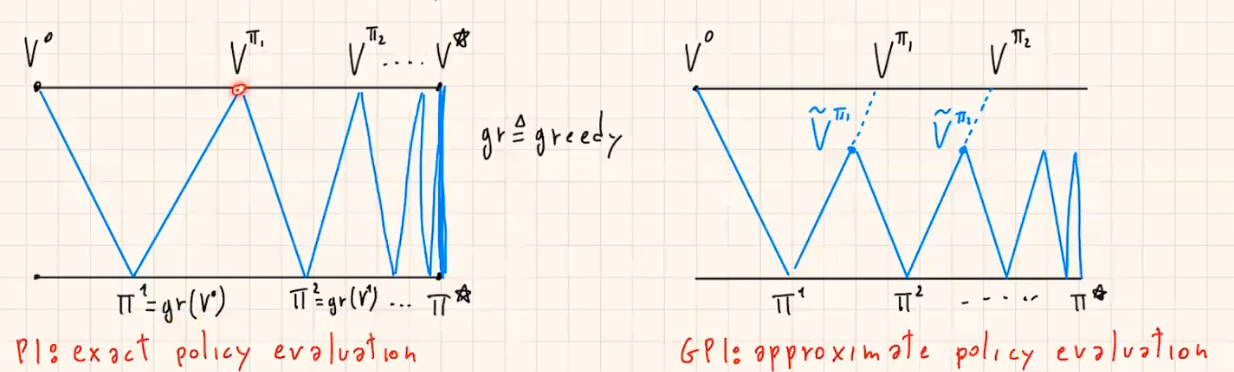
\includegraphics[width = .9\textwidth]{image0304}
\end{figure}

This class of methods is called Actor-Critic because the value function is called \side{critic} given that it evaluates the policy, which is called \side{actor}, in order to improve it.

Moreover, this class of methods is on-policy, therefore the policy that you are using to act/choose the control inputs must be the same policy that you want to evaluate. However, this is not completely true since there is always the need for exploration, so you cannot just act greedly w.r.t. the value, there must be some kind of exploration mechanism.

For this reason, the policy used to generate transitions is typically not the same that is evaluated and improved.
\begin{itemize}
\item The \side{behavior policy} mixes a small amount of exploration into the \side{tarket policy}
\end{itemize}

The key difference between GPI and PI is that in GPI there is no guarantee that at each iteration is going to be a bit better then the previous one (GPI can generate policies that are worse than previous ones).

\subsubsection{SARSA: policy evaluation}
Let us now investigate a specific algorithm that falls into this class, called \side{SARSA}.

The name comes from the notation that it is used into reinforcement learning:
\begin{itemize}
\item the state $x$ is called state $s$
\item the control $u$ is called action $a$
\item the cost $l$ is called reward $r$
\end{itemize}

Since at each iteration we observe of keep track of the tuple:
\begin{gather*}
(x,u,l,x',u')\\
(s,a,r,s,a)
\end{gather*}

The key idea of SARSA is to exploit TD(0) in order to learn Q from on-policy samples (since we are estimating the value of the policy who uses $u'$).

Tipically an $\epsilon$-greedy policy is utilized to act and at each transition you collect a tuple with the initial state and control, the cost and the next state and control. You use this information in order to update the estimate of the Q function according to the following expression:
\begin{align*}
\delta(Q) &= l(x,u) + \gamma Q(x',u') - Q(x,u)\\
Q_{k+1}(x,u) &= Q_k(x,u) + \alpha_k\delta(Q_k)
\end{align*}

\begin{itemize}
\item It is very similar to Q learning, but it uses $Q(x',u')$ instead of $\min_{z} Q(x', z)$.
\item if $\pi$ was fixed you would obtain the same equation as temporal difference learning.
\item we are constrained to use TD(0), we can extend the algorithm to TD(N) or TD($\lambda$).
\item as TD, SARSA can diverge in off-policy situations
\end{itemize}


\subsubsection{SARSA: policy improvement}
We have different options available:
\begin{enumerate}
\item The simplest one is to take the policy that is greedy w.r.t. Q, since a greedy policy can be computed on the fly, because for each state that we need to choose a control input for we can just look at the Q for that state, look at all the value of Q for all the control inputs and choose the one that minimizes Q.
\item Use $\epsilon-$ greedy as behavior policy to ensure exploration.
\end{enumerate}

Even for SARSA we have some guarantee of convergence to $Q^*(x,u)$ if:
\begin{itemize}
\item \side{Greedy in the Limit with Infinite Exploration (GLIE)}.

This means that the algorithm is allowed not to be greedy in the limit, but as time goes towards infinity the policy needs to tend towards a greedy policy and we need to have infinite exploration.

Formally:
\begin{itemize}
\item All state-control pairs are visited infinitely many times
\item Policy converges to a greedy policy, e.g.:
\[\epsilon_k = \cfrac{1}{k}\]
\end{itemize}
\item \side{Robbins-Monro (RM) conditions} sequence of step sizes:
\[\sum_{k=1}^{\infty} \alpha_k = \infty \qquad;\qquad \sum_{k=1}^{\infty} \alpha_k^2 < \infty\]
\end{itemize}

Summary:
\begin{table}[!h]
\centering
\begin{NiceTabular}[hvlines]{cc}
\textbf{DP}&\textbf{TD}\\
\makecell{Policy Evaluation\\\\$V(x) = l+\gamma V(x')$} \rule[-1.1cm]{0pt}{2.5cm} & \makecell{TD Learning\\\\$V(x)\xleftarrow{\alpha} l +\gamma V(x')$}\\
\makecell{Policy Iteration\\\\$V(x) = l+\gamma V(x')$\\$\pi(x)= \argmin_u l + \gamma V(x'(u))$} \rule[-1.1cm]{0pt}{2.5cm} & \makecell{Sarsa\\\\$Q(x,u)\xleftarrow{\alpha} l +\gamma Q(x', u')$\\$\pi(x) = \argmin_u Q(x,u)$}\\
\makecell{Value Iteration\\\\$V(x) =\min_u l + \gamma V(x'(u))$} \rule[-1.1cm]{0pt}{2.5cm} & \makecell{Q-Learning\\\\$Q(x,u)\xleftarrow{\alpha} l +\gamma \min_{u'} Q(x',u')$}
\end{NiceTabular}
\end{table}

\section{Value function Approximator}
The problem with the algorithms of Model Free Control is that we assumed the MDP to be discrete (i.e. state and control spaces are discrete) which makes this spaces very very large if you want to apply them to real problems.

Discrete-space algorithms do not scale to large systems
\begin{itemize}
\item{\makebox[3cm]{Backgammon:\hfill} $10^{20}$ states}
\item{\makebox[3cm]{Go:\hfill} $10^{170}$ states}
\item{\makebox[3cm]{Robot:\hfill} continuous state space}
\end{itemize}
In all these cases there are too many states/controls to store and learn.

In order to solve this problem: instead of representing the value or Q function with a table or an array we can use function approximation techniques in order to approximate these functions
\[\hat{V}(x,w) \approx V_{\pi}(x)\qquad,\qquad \hat{Q}(x,u,w) \approx Q_{\pi}(x,u)\]
where $w$ are the parameters of the function.

This function approximation are nothing more than parametric functions, so the learning process aims to learn the function parameters such that the function approximator reseambles the actual functions and, as a consequence, reduce the size of the vector that you work with.


\subsection{Types of value function approximation}

\begin{minipage}{0.3\textwidth}
\centering
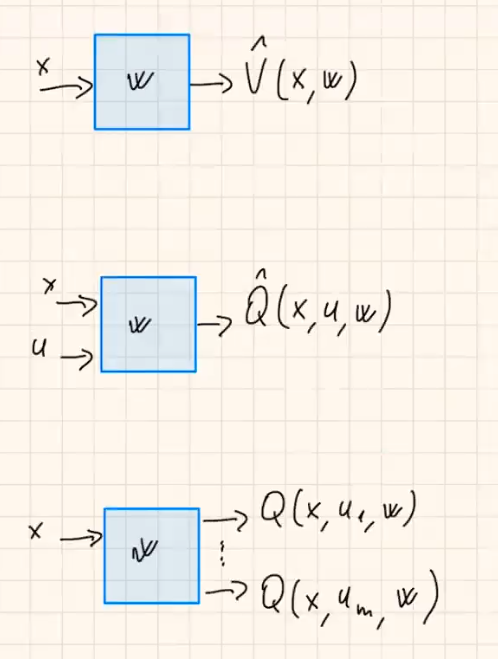
\includegraphics[width = .95\textwidth]{image0305}
\end{minipage}
\hfill
\begin{minipage}{.7\textwidth}
First of all both Q and/or V can be learnt:
\begin{enumerate}
\item You can learn the Value function by tuning the parameters of the function approximator, by providing as input the state $x$
\item You can learn the Q function by tuning the parameters of the function approximator, by providing as input both state $x$ and control $u$
\item You can parametrize the Q function, in the case of discrete control space, by providing as input only the state $x$, obtaining several output each of which corresponds to each possible value of the control input $u_1, ..., u_m$.
\end{enumerate} 

\end{minipage}

Very often, in the context of RL, the kind of value function approximators that are used are \side{Neural Networks}.

However any differential approximator can be used:
\begin{itemize}
\item linear combination of features (arbitrary functions of the state)
\item Fourier basis
\item Polynomials
\end{itemize}








